\documentclass{beamer}
\usepackage{beamerthemesplit}
\usepackage{wrapfig}
\usetheme{SPbGU}
\usepackage{pdfpages}
\usepackage{amsmath}
\usepackage{cmap} 
\usepackage[T2A]{fontenc} 
\usepackage[utf8]{inputenc}
\usepackage[english,russian]{babel}
\usepackage{indentfirst}
\usepackage{amsmath}
\usepackage{tikz}
\usepackage{multirow}
\usepackage[noend]{algpseudocode}
\usepackage{algorithm}
\usepackage{algorithmicx}
\usetikzlibrary{shapes,arrows}
\usepackage{fancyvrb}
\usepackage{tikz}
\usepackage{pgfplots}
\pgfplotsset{compat=1.9}
\newtheorem{rutheorem}{Теорема}
\newtheorem{ruproof}{Доказательство}
\newtheorem{rudefinition}{Определение}
\newtheorem{rulemma}{Лемма}
\beamertemplatenavigationsymbolsempty

\title[]{Поддержка конъюнктивных грамматик в GLL}
\institute[СПбГУ]{
Санкт-Петербургский государственный университет \\
Кафедра системного программирования }

\author[Горохов Артем]{Горохов Артем Владимирович, 371 группа \\
  \and  
    {\bfseries Научный руководитель:} магистр ИТ, ст.пр. С.В. Григорьев}

\date{26 мая 2016г.}

\begin{document}
{
\begin{frame}
  \begin{center}
  {
\includegraphics[width=1.5cm]{courseworkpictures/SPbGU_Logo.png}}
  \end{center}
  \titlepage
\end{frame}
}

\begin{frame}[fragile]
  \transwipe[direction=90]
  \frametitle{Введение}
  \begin{itemize}
    \item Расширение класса распознаваемых языков 
    \item Пример использования: поиск транспортных РНК
  \end{itemize}
\end{frame}
            
\begin{frame}
  \transwipe[direction=90]
  \frametitle{Обзор}
  \begin{itemize}
    \item Generalised LL
    \item Конъюнктивные грамматики \\
        \centerline{Грамматика для контекстно-зависимого языка \{$a^n b^n c^n, n \geq 0$\}} \\
        \\
        \vspace{-10pt}
        \\
        $$
        \begin{array}{crcl}
        & \mbox{\texttt{ S }} &::=& \mbox{\texttt{ A B }} \& \mbox{\texttt{ D C}} \\
        & \mbox{\texttt{ A }} & ::=& \mbox{\texttt{ a A |}}  \epsilon \\
        & \mbox{\texttt{ B }} & ::=& \mbox{\texttt{ b B c |}}  \epsilon \\
        & \mbox{\texttt{ C }} & ::=& \mbox{\texttt{ c C |}}  \epsilon \\
        & \mbox{\texttt{ D }} & ::=& \mbox{\texttt{ a D b |}}\epsilon \\
        \end{array}
        $$
    \item YaccConstructor
  \end{itemize}
\end{frame}

\begin{frame}
  \transwipe[direction=90]
  \frametitle{Цель и задачи}
  \textbf{Целью} работы является добавление поддержки конъюнктивных грамматик в YассConstructor  

  \textbf{Задачи}:
  \begin{itemize}
    \item Реализовать поддержку конъюнктивных грамматик в языке YARD
    \item Реализовать поддержку конъюнктивных грамматик в генераторе GLL-анализаторов
    \item Провести экспериментальные исследования работы алгоритма
  \end{itemize}
\end{frame}

\begin{frame}
  \transwipe[direction=90]
  \frametitle{Архитектура}
  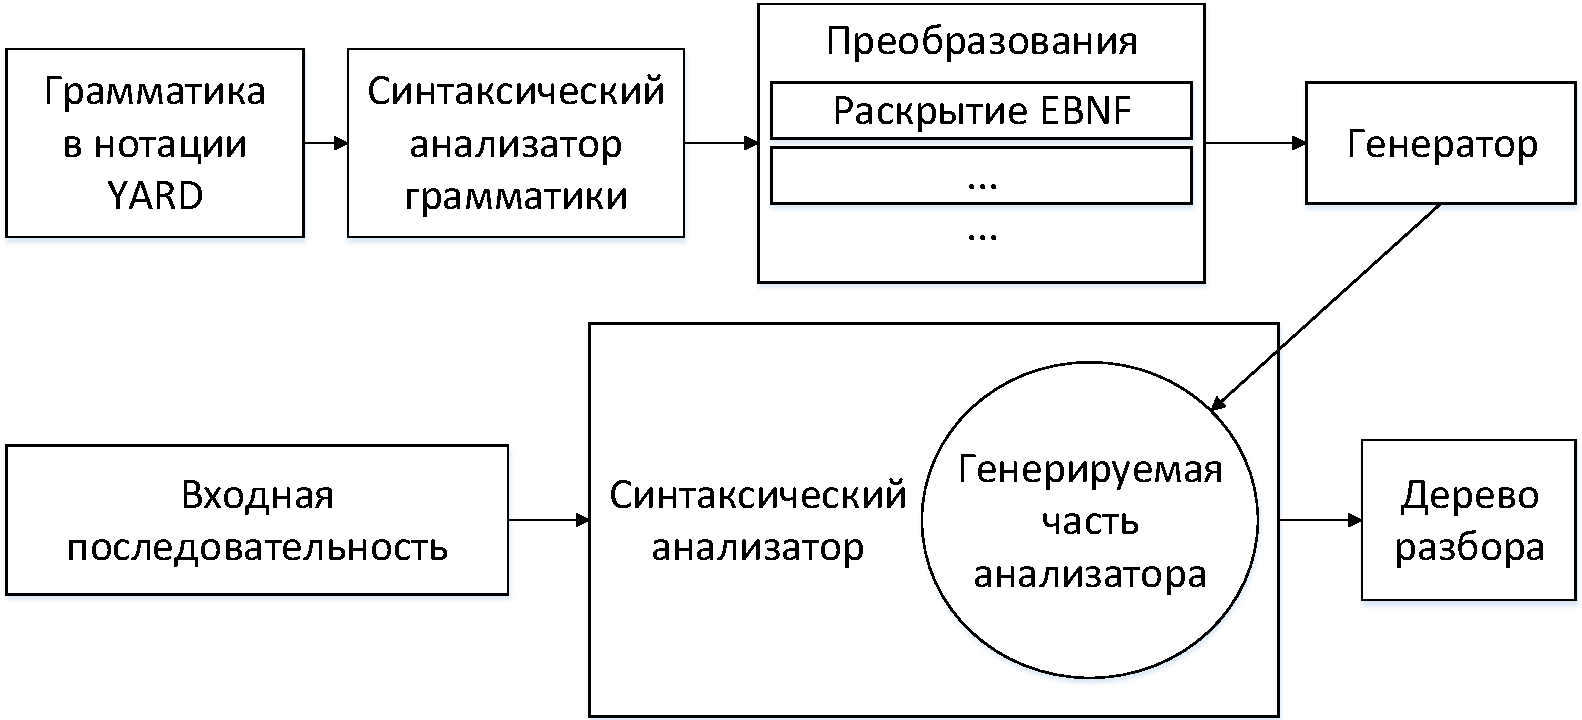
\includegraphics[width=12cm]{courseworkpictures/img2.pdf}
\end{frame} 

\begin{frame}
  \transwipe[direction=90]
  \frametitle{Решение}
  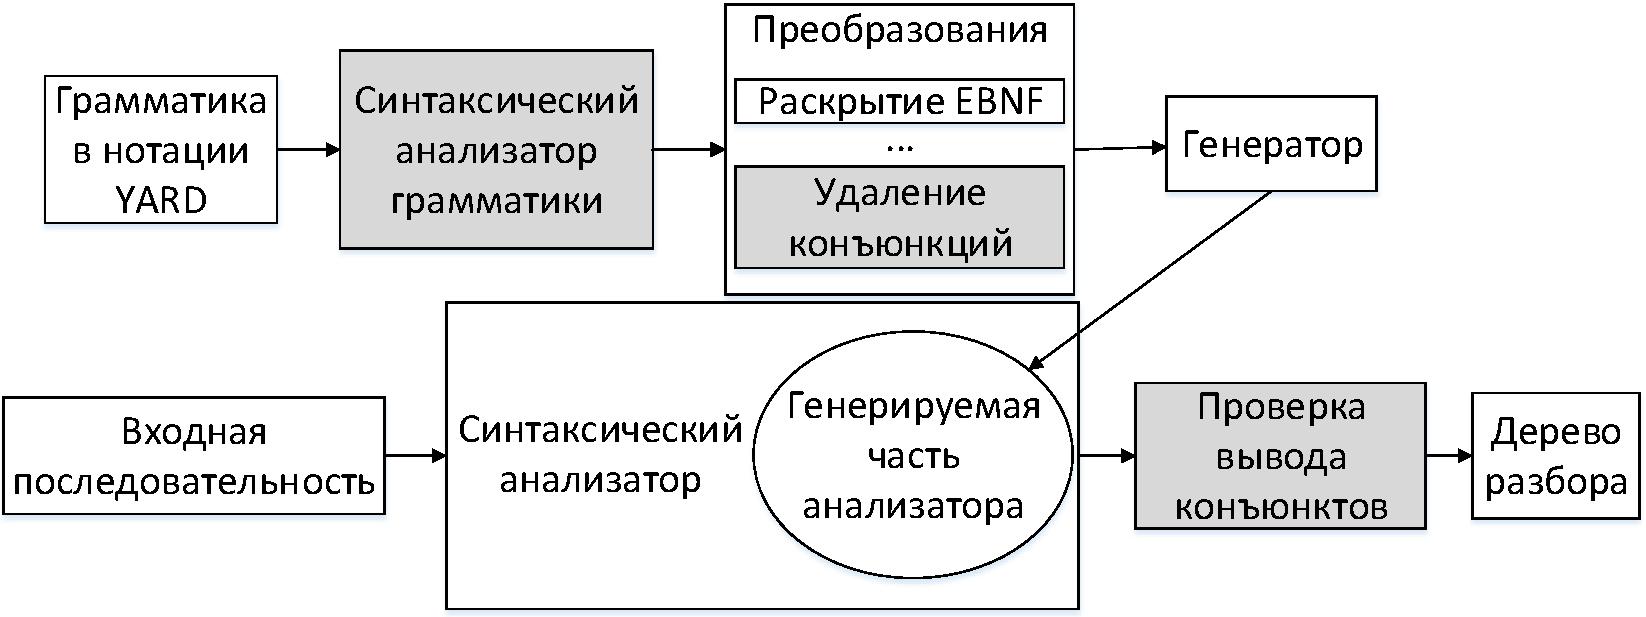
\includegraphics[width=12cm]{courseworkpictures/img3.pdf}
\end{frame}

\begin{frame}
  \transwipe[direction=90]
  \frametitle{Эксперименты}
  \begin{figure}
    \begin{center}
    \begin{tikzpicture}
    \begin{axis}[
        legend pos = north west,
	    xlabel = {Количество лексем},
	    ylabel = {Время, с}
        ]
    \addplot coordinates {
	    (100,2) (200,17) (300,42) (400,81) (500,128) (600,190) (700,264) (800,345) (900,446) (1000,562)
    };
    \addplot coordinates {
	    (100,1) (200,2) (300,4) (400,8) (500,12) (600,18) (700,22) (800,28) (900,36) (1000,43)
    };
    \legend{ 
	    конъюнктивная грамматика, 
	    КС-грамматика
    };
    \end{axis}
    \end{tikzpicture}
    \vspace{-13pt}
    \caption{Среднее время работы алгоритма на конъюнктивной и контекстно-свободной грамматиках тРНК}
    \label{time}
    \end{center}
    \end{figure}
\end{frame} 

\begin{frame}
  \transwipe[direction=90]
  \frametitle{Эксперименты}
  \begin{table}
  \begin{center}
  \begin{tabular}{ | c | c | c |}
    \hline
     & КС-грамматика & Конъюнктивная грамматика \\ \hline
    Тест 1 & 15 & 0 \\\hline
    Тест 2 & 5 & 0 \\\hline
    Тест 3 & 11 & 0 \\
    \hline
  \end{tabular}
  \caption{Количество некорректных цепочек, распознанных синтаксическим анализатором}
  \label{mistakes}
  \end{center}
  \end{table}
\end{frame} 

\begin{frame}
  \transwipe[direction=90]
  \frametitle{Результаты}
  \begin{itemize}
    \item Реализована поддержка конъюнктивных грамматик в языке YARD
    \item Реализована поддержка конъюнктивных грамматик в генераторе GLL-анализаторов
    \item Проведены экспериментальные исследования работы алгоритма
  \end{itemize}
\end{frame}

\end{document}
